\section{Auswertung}
\label{sec:Auswertung}

\subsection{Matrixrechnung}

Die Matrix $\underline{\underline{A}}$ aus Gleichung \ref{eqn:matrixA} für die Projektionen $I_j$ aus Abbildung \ref{fig:Aufbau2} hat die Form 

\begin{align}
  \underline{\underline{A}} = \left[\begin{matrix}0 & \sqrt{2} & 0 & \sqrt{2} & 0 & 0 & 0 & 0 & 0\\0 & 0 & \sqrt{2} & 0 & \sqrt{2} & 0 & \sqrt{2} & 0 & 0\\0 & 0 & 0 & 0 & 0 & \sqrt{2} & 0 & \sqrt{2} & 0\\1 & 1 & 1 & 0 & 0 & 0 & 0 & 0 & 0\\0 & 0 & 0 & 1 & 1 & 1 & 0 & 0 & 0\\0 & 0 & 0 & 0 & 0 & 0 & 1 & 1 & 1\\0 & \sqrt{2} & 0 & 0 & 0 & \sqrt{2} & 0 & 0 & 0\\\sqrt{2} & 0 & 0 & 0 & \sqrt{2} & 0 & 0 & 0 & \sqrt{2}\\0 & 0 & 0 & \sqrt{2} & 0 & 0 & 0 & \sqrt{2} & 0\\0 & 0 & 1 & 0 & 0 & 1 & 0 & 0 & 1\\0 & 1 & 0 & 0 & 1 & 0 & 0 & 1 & 0\\1 & 0 & 0 & 1 & 0 & 0 & 1 & 0 & 0\end{matrix}\right].
\end{align}

Damit menschliche Rechenfehler vermieden werden, werden alle Matrixrechnungen, auch Inversion und Transposition, in den folgenden Abschnitten mit dem Python-Modul \texttt{sympy} \cite{sympy} bearbeitet. Das Python-Modul \texttt{sympy} ist ein Computeralgebrasystem zum Rechnen mit symbolischen Ausdrücken. 

 
\subsection{Spektrum der $^{137}Cs$-Quelle}

Für die bestimmung der Prozesse in dem Messpektrum wurden die gemessenen Ereignisse am $NaJ$-Detektor grafisch gegen die Channels dargestellt in Abbildung \ref{fig:leer}. Bei dieser Messung war der erste Würfel zwischen $\gamma$-Quelle und Detektor. 
\begin{figure}[H]
  \centering
  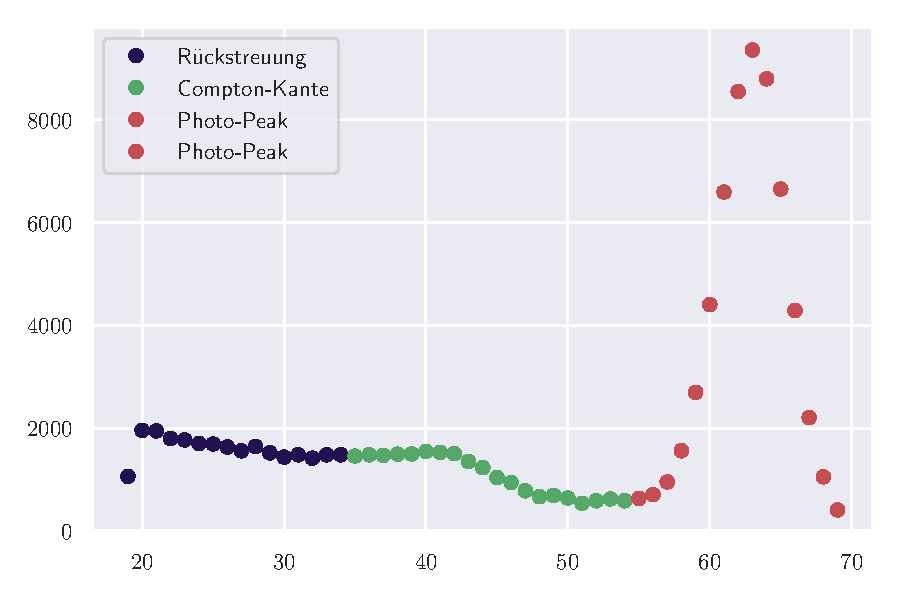
\includegraphics[width = 0.9 \textwidth]{Daten/leerlauf.pdf}
  \caption{Die identifizierten Prozesse in dem Spektrum der Messung der $^{137}Cs$-Quelle. Die Quelle strahlt bei dieser Messung durch die Hauptdiagonale des leeren Würfels. }
  \label{fig:leer}
\end{figure}

In der Abbildung \ref{fig:leer} sind die erkannten Prozesse im Spektrum eingezeichnet. Der Photo-Peak befindet sich im Channel $62.44$. Nach der Literatur liegt dieser Punkt bei der Energie $E_P = 661.7 \,\si{\kilo\electronvolt}$ \cite{CS_Peak}. 
 
\subsection{Würfel 1}

Um die Untergrundstrahlung zu messen, wird für die Nullmessung der Intensität ein leerer Würfel verwendet, der die Nummerierung 1 beträgt und aus einem Aluminiummantel besteht. Diese wird in den Messungen jeweils automatisch vom gemessenen Spektrum abgezogen. 
Aufgrund der unterschiedlichen Dicken bei den verschiedenen Einstrahlungswinkel werden einmal die diagnoalen Strahlengänge $I_7$ und $I_8$ sowie der horizontale Strahlengang $I_4$ 
gemessen. Die Messwerte dazu befinden sich in der Tabelle \ref{tab:w1}.
\begin{table}[H]
  \centering
  \begin{tabular}{c c c c}
    \toprule
     Projektion &  $t \:/\: \si{\second}$ &                   $N$ &           $I \:/\: \si{\per\second}$ \\
    \midrule
              $I_{4}$ &   $300$ & $49176\pm 306$ & $163.9\pm 1.0$ \\
              $I_{7}$ &   $300$ & $48599\pm 320$ & $162.0\pm 1.1$ \\
              $I_{8}$ &   $300$ & $48599\pm 320$ & $162.0\pm 1.1$ \\
    \bottomrule
  \end{tabular}
  \caption{Die gemessenen Net-Areas des Photo-Peaks und die entsprechende Zählraten des leeren Würfels, welcher nur aus der Aluminiumhülle besteht}
  \label{tab:w1}
\end{table}

Die Counts $N$ wurden hierbei im Messprogramm unter der Variable \texttt{Net Area} angegeben. Die Variable \texttt{Net Area} setzt sich so zusammen, dass alle Ereignisse im Photo-Peak integriert werden und der Untergrund automatisch subtrahiert wird. 
Der Fehler der Counts ist statistisch verteilt und hat die Form 
\begin{align*}
  \sigma_N = \sqrt{N}.
\end{align*}
Die Zeit ist zwar auch fehlerbehaftet aber da diese am Computer gemessen wird und dieser die Zeit in Millisekunden genau messen kann, ist der Fehler in der Zeit bei den Messungen in diesem Versuch sehr klein und daher vernachlässigbar. \\
Die Intensitäten werden mit der folgenden Gleichung berechnet: \begin{align*}
  I = \frac{N}{t}
\end{align*}
und der Fehler der Intensität wird nach der gaußschen Fehlerfortpflanzung vereinfacht zu 
\begin{align*}
  \sigma_I = \frac{\sigma_N}{t}.
\end{align*}
Die gemessenen Intensitäten in diesem Abschnitt werden im weiteren Verlauf als Intensität $I_0$ verwendet, die den Hohlwürfel passieren. 


\subsection{Würfel 2}
Die Messwerte für den Würfel 2 befinden sich in der Tabelle \ref{tab:w2}. Die Absorptionskoeffizienten werden mit der Gleichung \ref{eqn:mu_full} berechnet, wobei die Diagonalelemente der Gewichtungsmatrix $\underline{\underline{W}}$ 
anhand der gaußschen Fehlerfortpflanzung also 
\begin{align}
  \sigma_{W_i} = \sqrt{(\frac{\sigma_{I_0}}{I_0})^2 + \frac{\sigma_{N_j}}{N_j})^2}
\end{align}
berechnet werden. Die berechneten Absorptionskoeffizienten sind in der Tabelle \ref{tab:w2_mu} angegeben. 
\begin{table}[H]
  \centering
  \begin{tabular}{c c c c}
    \toprule
     Projektion &  $t \:/\: \si{\second}$ &     $N$ &           $N_j \:/\: \si{\per\second}$ \\
    \midrule
            $I_{  4}$ &   $300$ & $41777 \pm    300$ & $139.3\pm1.0$ \\
            $I_{  5}$ &   $300$ & $43230 \pm    289$ & $144.1\pm1.0$ \\
            $I_{  6}$ &   $300$ & $41772 \pm    287$ & $139.2\pm1.0$ \\
            $I_{  7}$ &   $300$ & $43714 \pm    273$ & $145.7\pm0.9$ \\
            $I_{  8}$ &   $300$ & $42274 \pm    259$ & $140.9\pm0.9$ \\
            $I_{  9}$ &   $300$ & $41326 \pm    297$ & $137.8\pm1.0$ \\
            $I_{ 12}$ &   $300$ & $41886 \pm    297$ & $139.6\pm1.0$ \\
            $I_{ 11}$ &   $300$ & $42662 \pm    288$ & $142.2\pm1.0$ \\
            $I_{ 10}$ &   $300$ & $44080 \pm    280$ & $146.9\pm0.9$ \\
    \bottomrule
    \end{tabular}
  \caption{Die gemessenen Net-Areas des Photo-Peaks und die entsprechenden Intensitäten des zweiten Würfels. }
  \label{tab:w2}
\end{table}

\begin{table}[H]
  \centering
  \begin{tabular}{c c}
    \toprule
     $\mu_k$ &  $\mu \:/\: \si{\per\centi\metre}$ \\
    \midrule
            $\mu_{  1}$ &   $-0.601181$ \\
            $\mu_{  2}$ &   $ 1.451370$ \\
            $\mu_{  3}$ &   $ 0.631905$ \\
            $\mu_{  4}$ &   $ 1.545090$ \\
            $\mu_{  5}$ &   $ 0.429356$ \\
            $\mu_{  6}$ &   $-0.093726$ \\
             $\mu_{ 7}$ &   $ 0.623833$ \\
             $\mu_{ 8}$ &   $ 0.866272$ \\
             $\mu_{ 9}$ &   $ 0.265099$ \\
    \bottomrule
    \end{tabular}
  \caption{Berechnete Absorptionskoeffizienten für den zweiten Würfel. }
  \label{tab:w2_mu}
\end{table}


\begin{align}
  \bar{\mu}_2 = 0.57\pm 0.22 \,\si{\centi\metre}
\end{align}
\subsection{Würfel 3}

\begin{table}[H]
  \centering
  \begin{tabular}{c c c c}
    \toprule
    Projektion &  $t \:/\: \si{\second}$ &     $N$ &           $N_j \:/\: \si{\per\second}$ \\
    \midrule
             $I_{ 4}$ &   $300$ & $1788 \pm   55$ & $5.96\pm0.18$ \\
             $I_{ 5}$ &   $300$ & $1751 \pm   56$ & $5.84\pm0.19$ \\
             $I_{ 6}$ &   $300$ & $2148 \pm   58$ & $7.16\pm0.19$ \\
             $I_{ 7}$ &   $300$ & $1928 \pm   60$ & $6.43\pm0.20$ \\
             $I_{ 9}$ &   $300$ & $2689 \pm   62$ & $8.96\pm0.21$ \\
             $I_{ 8}$ &   $300$ & $1358 \pm   72$ & $4.53\pm0.24$ \\
             $I_{12}$ &   $300$ & $2145 \pm   60$ & $7.15\pm0.20$ \\
             $I_{11}$ &   $300$ & $1829 \pm   60$ & $6.10\pm0.20$ \\
             $I_{10}$ &   $300$ & $1904 \pm   60$ & $6.35\pm0.20$ \\
    \bottomrule
  \end{tabular}
  \caption{Die gemessenen Net-Areas des Photo-Peaks und die entsprechende Zählraten des dritten Würfels. }
  \label{tab:w3}
\end{table}


\begin{table}[H]
  \centering
  \begin{tabular}{c c}
    \toprule
     $\mu_k$ &  $\mu \:/\: \si{\per\centi\metre}$ \\
    \midrule
            $\mu_{  1}$ &   $-0.080$ \\
            $\mu_{  2}$ &   $ 0.164$ \\
            $\mu_{  3}$ &   $ 0.025$ \\
            $\mu_{  4}$ &   $ 0.096$ \\
            $\mu_{  5}$ &   $ 0.005$ \\
            $\mu_{  6}$ &   $-0.074$ \\
             $\mu_{ 7}$ &   $ 0.026$ \\
             $\mu_{ 8}$ &   $-0.108$ \\
             $\mu_{ 9}$ &   $ 0.124$ \\
    \bottomrule
    \end{tabular}
  \caption{Berechnete Absorptionskoeffizienten für den dritten Würfel. }
  \label{tab:w3_mu}
\end{table}


\begin{align}
  \bar{\mu}_3 = 0.020\pm0.030 \,\si{\centi\metre}
\end{align}

\subsection{Würfel 4}


\begin{table}[H]
  \centering
  \begin{tabular}{c c c c}
    \toprule
    Projektion &  $t \:/\: \si{\second}$ &     $N$ &           $N_j \:/\: \si{\per\second}$ \\
    \midrule
        $I_{  4}$ &   $300$ & $14752 \pm     146$ & $  49.2\pm0.5$ \\
        $I_{  5}$ &   $300$ & $13959 \pm     170$ & $  46.5\pm0.6$ \\
        $I_{  6}$ &   $300$ & $13095 \pm     168$ & $  43.6\pm0.6$ \\
        $I_{  7}$ &   $300$ & $ 9203 \pm     140$ & $  30.7\pm0.5$ \\
        $I_{  8}$ &   $300$ & $ 8382 \pm     107$ & $  27.9\pm0.4$ \\
        $I_{  9}$ &   $300$ & $11430 \pm     194$ & $  38.1\pm0.6$ \\
        $I_{ 12}$ &   $300$ & $41959 \pm     274$ & $ 139.9\pm0.9$ \\
        $I_{ 11}$ &   $300$ & $ 1732 \pm      52$ & $  5.77\pm0.17$ \\
        $I_{ 10}$ &   $300$ & $40324 \pm     279$ & $ 134.4\pm0.9$ \\
        $I_{  1}$ &   $300$ & $ 9735 \pm     161$ & $  32.5\pm0.5$ \\
        $I_{  2}$ &   $300$ & $ 8366 \pm     104$ & $ 27.89\pm0.35$ \\
        $I_{  3}$ &   $300$ & $13498 \pm     170$ & $  45.0\pm0.6$ \\
      \bottomrule
  \end{tabular}
  \caption{Die gemessenen Net-Areas des Photo-Peaks und die entsprechende Zählraten des vierten Würfels. }
  \label{tab:w4}
\end{table}